%----------------------------------------------------------------------------------------
%	PACKAGES AND THEMES
%----------------------------------------------------------------------------------------
\documentclass[aspectratio=169,xcolor=dvipsnames]{beamer}
\usetheme{Simple}

\usepackage{hyperref}
\usepackage{graphicx} % Allows including images
\usepackage{booktabs} % Allows the use of \toprule, \midrule and \bottomrule in tables

%----------------------------------------------------------------------------------------
%	TITLE PAGE
%----------------------------------------------------------------------------------------

% The title
\title{Arch Linux}
\subtitle{Una distribuzione \emph{semplice}}

\author {Davide Carnemolla}
\institute % Your institution may be shorthand to save space
{
    % Your institution for the title page
    Dipartimento di Matematica e Informatica \\
    Università degli Studi di Catania
    \vskip 3pt
}
\date{\today} % Date, can be changed to a custom date


%----------------------------------------------------------------------------------------
%	PRESENTATION SLIDES
%----------------------------------------------------------------------------------------

\begin{document}

\begin{frame}
    % Print the title page as the first slide
    \titlepage
\end{frame}

\begin{frame}{Panoramica}
    % Throughout your presentation, if you choose to use \section{} and \subsection{} commands, these will automatically be printed on this slide as an overview of your presentation
    \tableofcontents
\end{frame}

%------------------------------------------------
\section{Cos'è una distribuzione GNU/Linux?}
%------------------------------------------------
\begin{frame}{GNU/Linux prima delle distribuzioni}
    \begin{itemize}
        \item Linux era distribuito solo come codice sorgente
        \item Chi voleva usare Linux doveva compilarlo da sé
        \item L'utilizzo era quindi accessibile solo agli sviluppatori
    \end{itemize}
    \hfill \break
    Per semplificare il processo di installazione e configurazione nascono le distribuzioni GNU/Linux.
\end{frame}

%------------------------------------------------

\begin{frame}{Le prime distribuzioni GNU/Linux}
    \begin{itemize}
        \item Boot-root - fine 1991
        \item MCC Interim Linux - 1992
        \item Slackware - 1993
        \item Yggdrasil Linux (Plug-and-Play) - 1993
    \end{itemize}
\end{frame}

\begin{frame}{Boot-root}
    \centering
    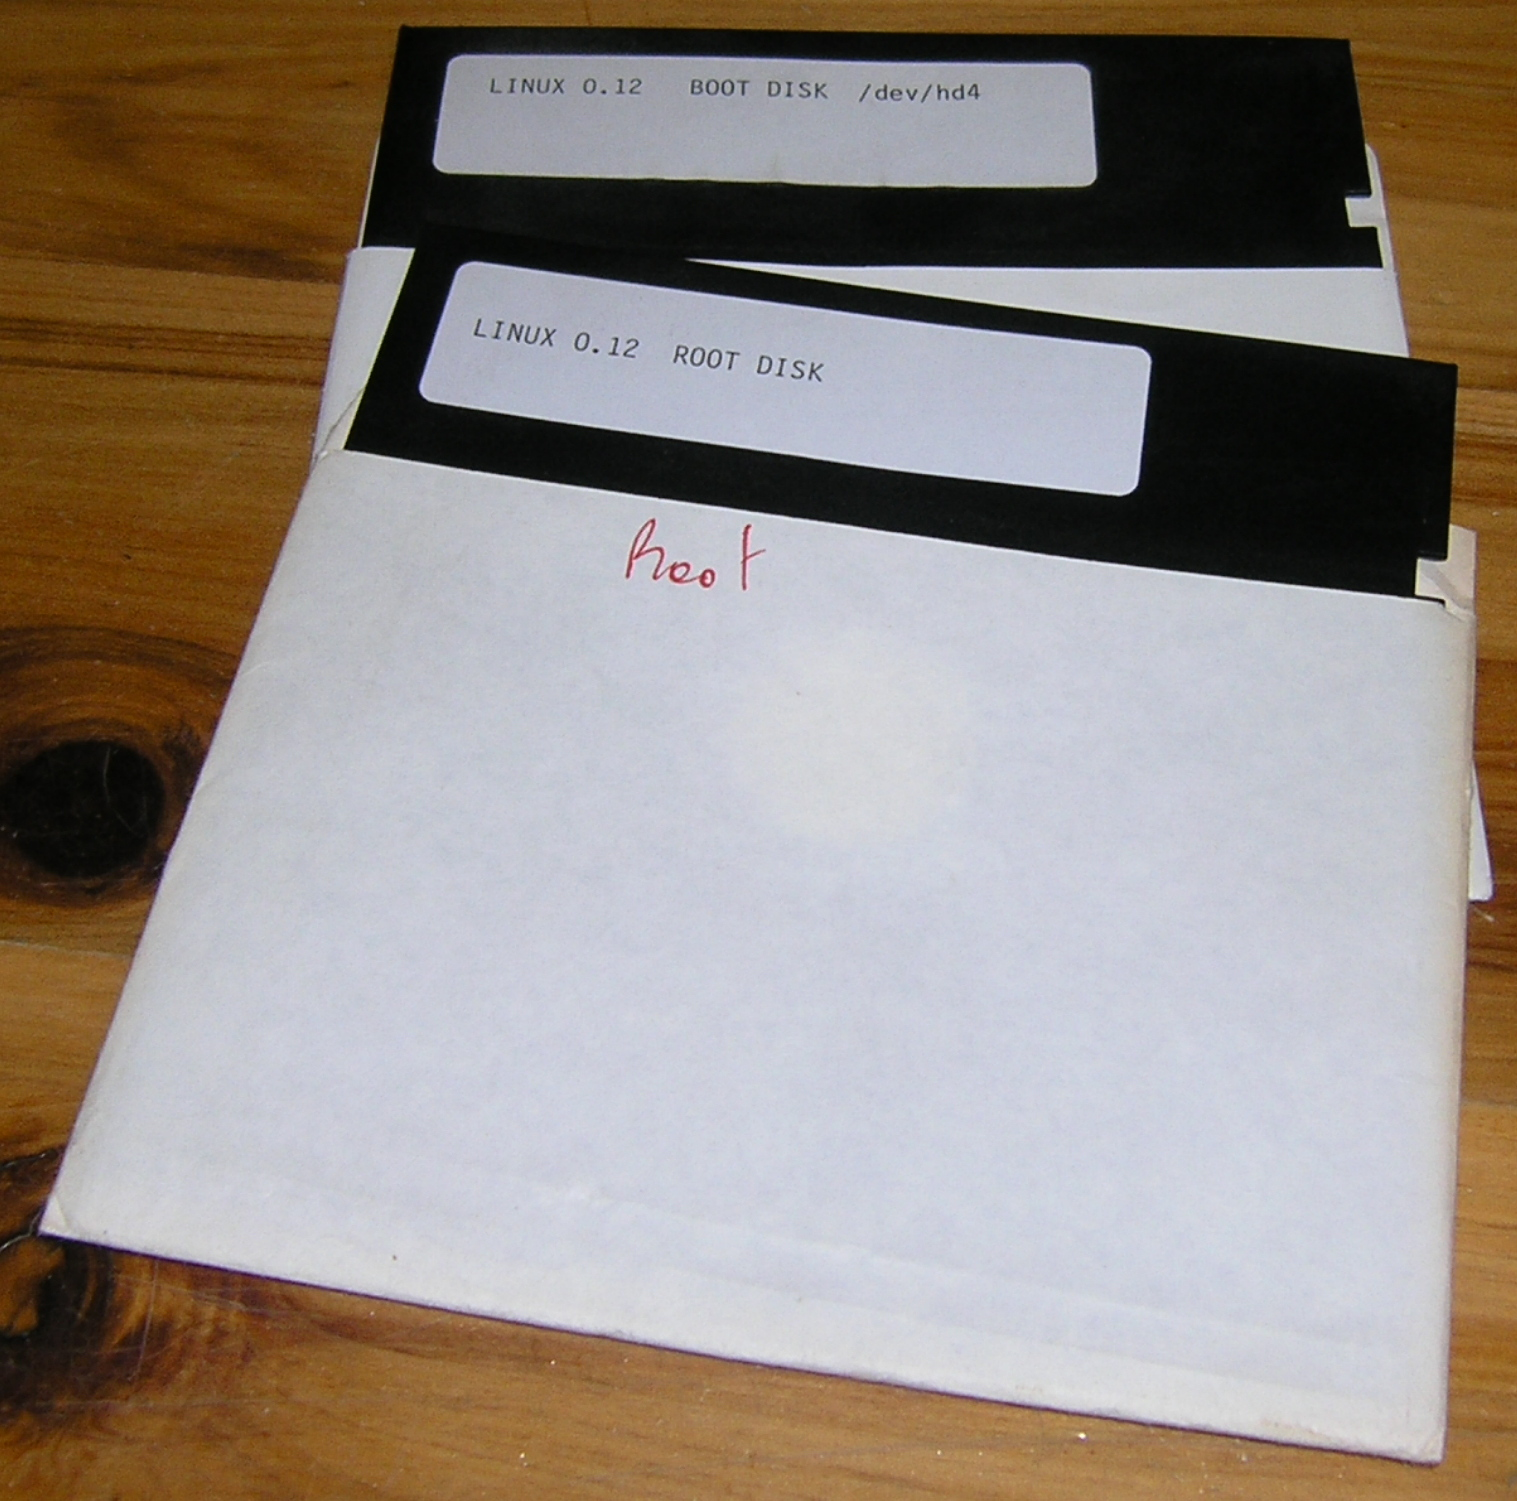
\includegraphics[scale=0.14]{images/Linux_0_12.jpg}
\end{frame}

%------------------------------------------------

\begin{frame}{Le distribuzioni GNU/Linux oggi}
    \centering
    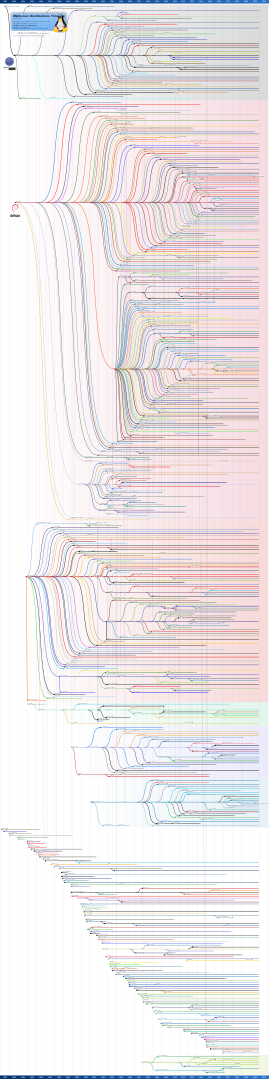
\includegraphics[scale=0.2]{images/Linux_Distribution_Timeline_Dec._2020.svg.png}
\end{frame}

\begin{frame}{Le distribuzioni GNU/Linux oggi}
    \centering
    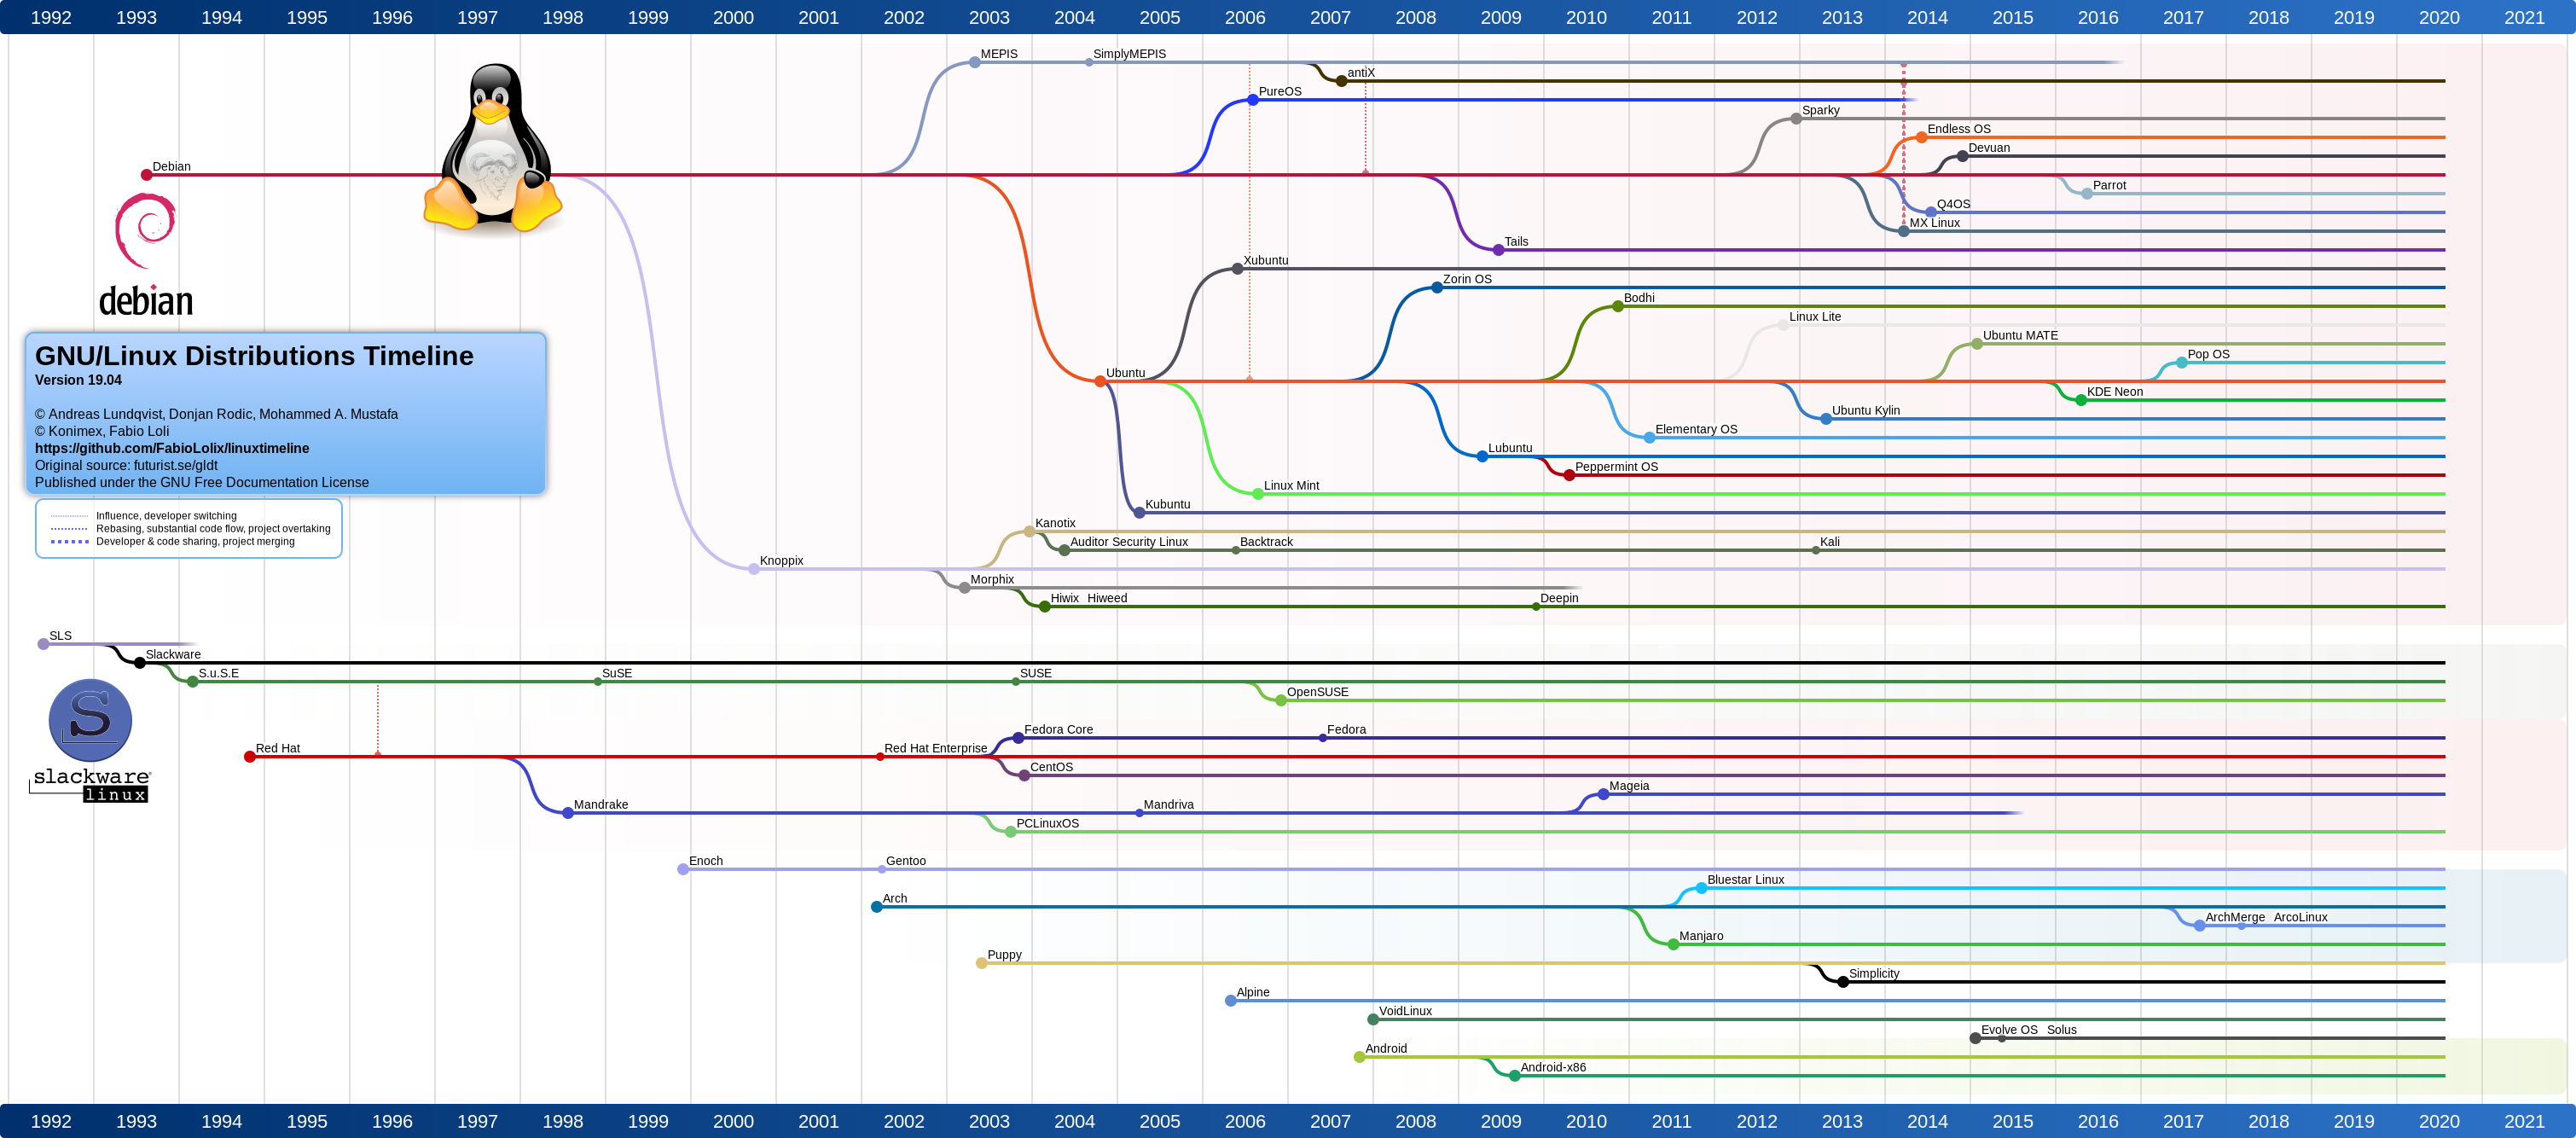
\includegraphics[scale=0.18]{images/aygzaivcbmd51.png}
\end{frame}

\begin{frame}{Le distribuzioni GNU/Linux oggi}
Possiamo suddividere le distribuzioni in GNU/Linux in famiglie:
\begin{itemize}
    \item Debian(Ubuntu, MX Linux, Kali Linux)
    \item Arch Linux(Manjaro, EndeavourOS)
    \item Fedora
    \item Gentoo
    \item ...
\end{itemize}

\end{frame}

%------------------------------------------------


\section{Cos'è Arch Linux?}
\begin{frame}{Arch Linux}
    \begin{figure}[h]
        
\includegraphics[width=0.2\textwidth]{images/Archlinux-icon-crystal-64.png}
    \end{figure}
    \textbf{Arch Linux} è una distribuzione GNU/Linux\\

    \begin{itemize}
        \item Creata da Judd Vinet nel 2002
        \item Basata sulla filosofia \textit{KISS}
        \item Inizialmente ispirata a \textit{CRUX Linux}
    \end{itemize}
\end{frame}

%-----------------------------------------------



\section{Installazione Arch Linux}
\begin{frame}{Installazione minimale di Arch Linux}
    Effettueremo un'installazione con la seguente configurazione:
    \begin{itemize}
        \item \textbf{Desktop Environment}: GNOME
        \item \textbf{Display Server}: Wayland
        \item \textbf{Filesystem}: ext4 (singola partizione)
        \item \textbf{Cifratura disco}: Nessuna
    \end{itemize}
\end{frame}

\begin{frame}{Serve aiuto?}
    \begin{itemize}
        \item Installation Guide(\url{https://wiki.archlinux.org/index.php/Installation_guide})
        \item Arch Official Wiki(\url{https://wiki.archlinux.org/})
        \item Arch Official Forum(\url{https://bbs.archlinux.org/})
        \item ...
    \end{itemize}
\end{frame}

\section{Strumenti Utili}
\begin{frame}{Strumenti utili}
    \begin{itemize}
        \item \textbf{pacman}
        \item \textbf{yay}
        \item \textbf{flatpak}
        \item \textbf{tlp} (Advanced power management for laptop)
    \end{itemize}
\end{frame}

\section{Conclusioni}
\input{Conclusioni}

\section{Contatti}
\begin{frame}{Contatti}
    \begin{itemize}
        \item \textbf{@Herbrant}(Github, Telegram, Discord)
        \item \textbf{email}: cdavide98carnemolla@gmail.com
    \end{itemize}
\end{frame}

%----------------------------------------------------------------------------------------

\end{document}
